\section{Experiments}

\subsection{Datasets}

In our experiments, we applied STL-10 \cite{singh2019justification}, CIFAR-10 \cite{ho2018cifar10} and SVHN \cite{sermanet2012convolutional} datasets for unlabeled RL training. The STL-10 dataset is specially designed for unsupervised feature learning as it contains $13,000$ labeled images across $10$ classes and $100,000$ unlabeled images. While we used the entire training set of CIFAR-10 and SVHN datasets for RL, we only used $250$, $1,000$, and $4,000$ labeled training samples in downstream classifications. Additional experiments were conducted on 6 other image datasets \cite{krizhevsky2009learning, xiao2017fashionmnist, LFWTech, helber2019eurosat, nilsback2008automated, imagenette2019} with different class numbers.

\subsection{Implementation Details} 

\textbf{Image augmentations:} We adopt an augmentation pipeline similar to SimCLR and BYOL, implemented in PyTorch \cite{paszke2019pytorch}. For geometric transformations, we apply ``RandomResizedCrop" with a scaling factor between \([0.2, 1.0]\) and ``RandomHorizontalFlip" to introduce random horizontal flips. Color augmentations include ``ColorJitter", which modifies brightness, contrast, and saturation by a maximum factor of \(0.4\), and hue by \(0.1\), applied with a probability of \(0.3\). We include ``RandomGrayscale" to convert images to grayscale with a probability of \(0.2\). For blurring, ``GaussianBlur" is applied, using a Gaussian kernel with a standard deviation sampled from \([1.0, 2.0]\), with a \(0.2\) probability. Finally, we normalize the input images using predefined mean and standard deviation values. 

Our experiments reveal that image resolution significantly affects accuracy; thus, we resize all images to \(256 \times 256\). In the PL phase, weak augmentations are applied to the noisy teacher model, involving random horizontal and vertical flips, each with a probability of \(0.25\).

\noindent
\textbf{Architecture:} We use ResNet18 \cite{ayyachamy2019medical}, a more computationally feasible network, designed for GPU computations. This ResNet18 architecture remains consistent across all settings, including representation learning, and pseudo labeling. The MLPs, projection, and prediction layers adhere to the parameters established by BYOL. In PL, the teacher and student networks are initialized from the ResNet18, pre-trained via RL.

\noindent
\textbf{Optimization:} The RL framework was optimized using the Adam optimizer \cite{zhang2018improved}, whereas PL employed the Stochastic Gradient Descent (SGD) optimizer \cite{gower2019sgd}, both with a learning rate set to $0.0003$. The auxiliary loss is weighted at \(0.5\). RL underwent training for $50$ epochs with a batch size of $128$, while PL was trained over $150$ epochs with a batch size of $16$.

\begin{figure}[!htbp]
    \centering
    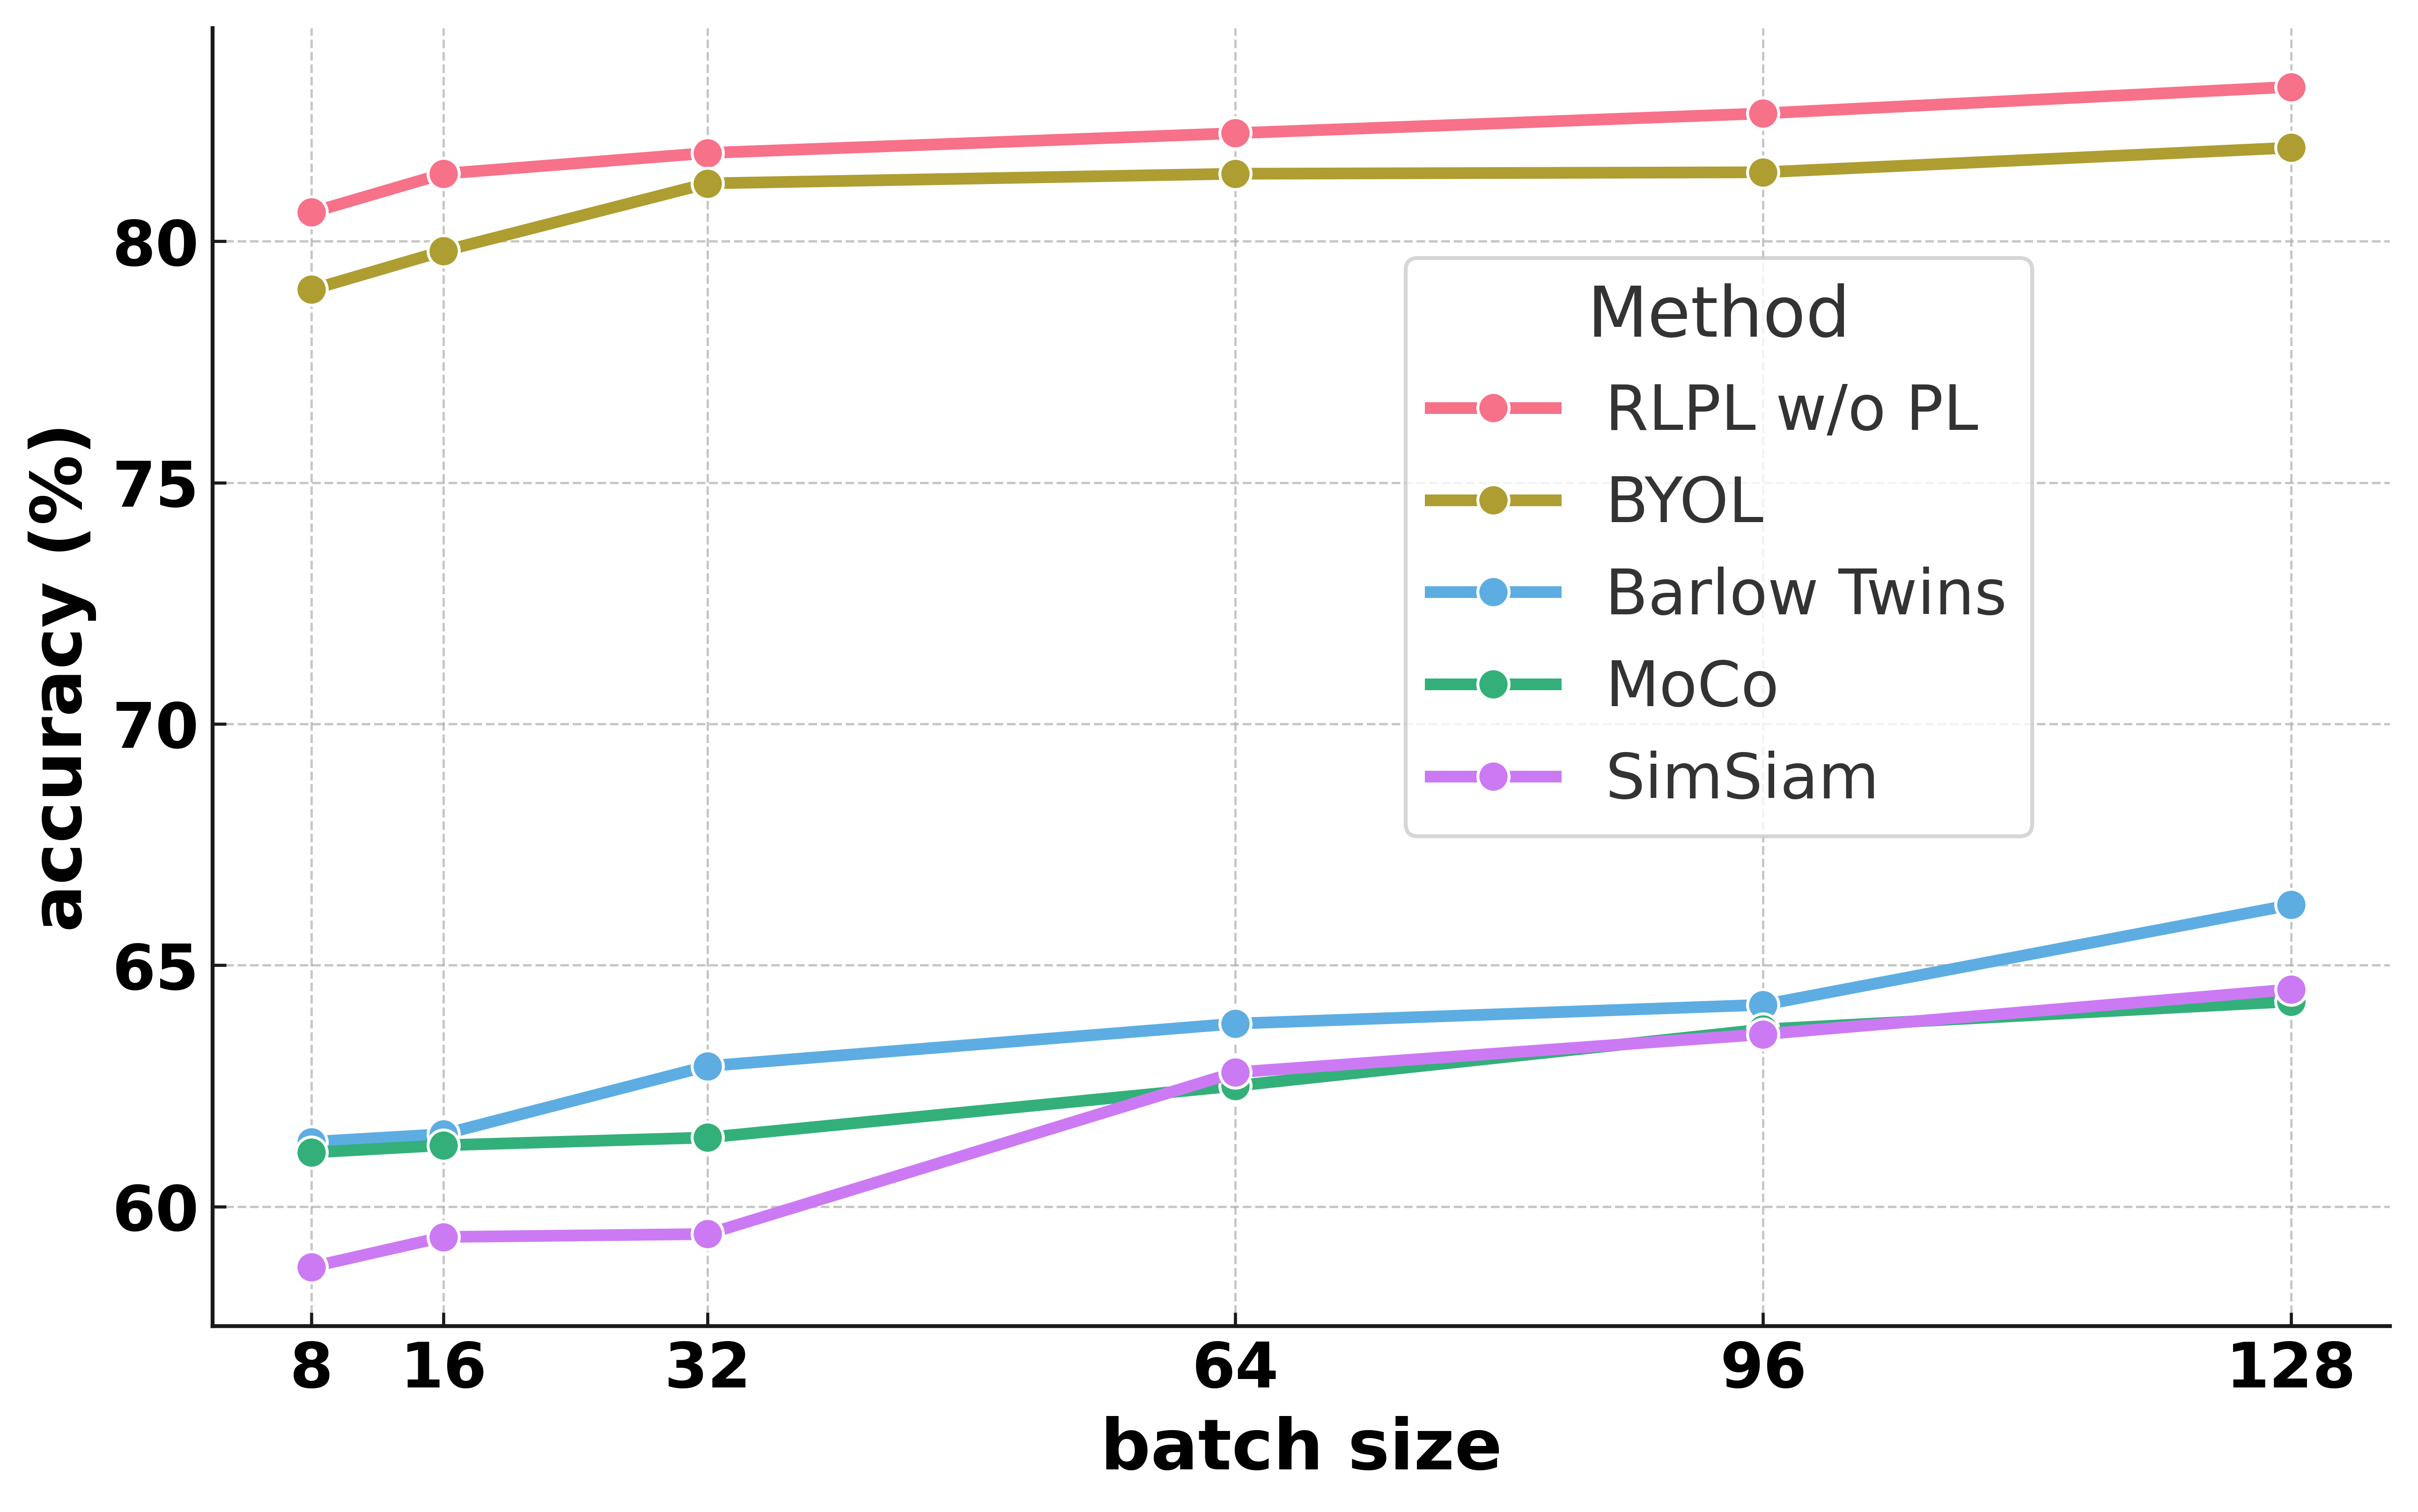
\includegraphics[width=0.9\columnwidth, keepaspectratio]{images/accuracy_vs_batch.png}
    \caption{Effect of batch size on model performance (evaluated on STL-10).}
    \label{fig:batch}
\end{figure}

\begin{table}[htbp]
    \centering
    \begin{tabular}{l c}
      \toprule
      \textbf{Methods} & \textbf{Test Accuracy (\%)} \\  
      \midrule
      Baseline (ResNet18) & 53.16 \\
      FixMatch \cite{sohn2020fixmatch} & 37.28 \\ 
      MixMatch \cite{berthelot2019mixmatch} & 71.60 \\
      MoCo & 66.25 \\
      SimSiam & 64.50 \\
      Barlow Twins & 64.25 \\
      BYOL & 81.94  \\
      RLPL (Ours) & \textbf{84.64} \\
      \bottomrule
    \end{tabular}
    \caption{Performance of different methods on STL-10 dataset.}
    \label{table:stl}
\end{table}
